

%src mongo lisence.


% https://www.techtarget.com/searchdatamanagement/definition/MongoDB
% jotain täältä. tämä tosin sanoo että on open source joka ei oo sinänsä totta
% sitaatti 28.5


%   TODO   TARKISTA KAIKKI VIITTEET ETTÄ NE OIKEESTI ON OIKEESTA PAIKASTA




%mongo website and repo
% 5.6

%https://www.mongodb.com/docs/manual/core/document/
%json bson, document format
% 5.6

%https://www.techtarget.com/searchdatamanagement/definition/MongoDB
% performance and availability
% 5.6

%https://www.mongodb.com/resources/products/fundamentals/why-use-mongodb
%used alot
% 5.6




MongoDB on NoSQL (eng "non sql"{} tai "not only sql"{}) dokumenttipohjainen tietokannan hallintaohjelma,
joka on MongoDB Inc:in valmistama ja ylläpitämä.
Se on suunniteltu käsittelemään suuria määriä strukturoimatonta dataa,
ja se tarjoaa suuren suorituskyvyn, korkean käytettävyyden ja helpon skaalautuvuuden\labciteend{alexander23}
\medskip




MongoDB tallentaa tiedot joustaviin, JSON-tyyppisiin dokumentteihin, 
joka tarkoittaa, että kentät voivat vaihdella dokumentista toiseen ja tietorakennetta voidaan muuttaa ajan myötä. \labcite{mongodb24a}
Tätä tietokantajärjestelmää käytetään laajalti nykyaikaisissa sovelluksissa, 
sillä se pystyy hallitsemaan erityyppisiä tietoja ilman kiinteää skeemaa\labciteend{mongodb24b}
\medskip








\subsubsection{Skaalautuminen}

%lenove sitaatit on fine paitsi ensimmäisessä lukee jotain outoo


%https://www.lenovo.com/us/en/glossary/scalling/
%6.6

Skaalautumisella tarkoitetaan sovelluksen, järjestelmän tai infrastruktuurin
mahdollisuutta hallita kasvavaa määrää dataa, käyttäjiä tai stressiä ilman että se kompormisoisi suorituskykyä tai vakautta.
Skaalautuminen on tärkeää sillä kun sovellus kasvaa, sen pitää pystyä käsittelemään kasvavaa kuormaa.
Ilman skaalautumista järjestelmästä voi tulla hidas tai se voi johtaa seisokkiaikaan.\labcite{lenovo}
\medskip

Vertikaalisella skaalautumisella tarkoitetaan yksittäisen palvelimen tai järjestelmän olemassa olevien resurssien kehittämistä, 
kuten keskusmuistin tai prosessorin päivitystä, kasvattaen järjestelmän kuorman hallintaa.\labcite{lenovo}
%mtextPP
\medskip

Horisontaali skaalaus käsittää koneiden ja järjestelmien lisäämistä, jotka pystyvät jakamaan kuorman usean palvelimen välillä.
Tämä tuo myös lisä turvaa sillä, jos järjestelmä tai sovellus kaatua palvelinvian takia, 
toinen palvelin voi tuurata sitä. \labcite{lenovo}
Mongodb skaalautuminen perustuu replikointi ja shardaus ominaisuuksiin, jotka toimivat horisontaalisella skaalautumisella.\labcite{mongodb24c} 
\medskip






MongoDB replikointi antaa mahdollisuuden tehdä varmuuskopioita tietokannasta ja säilyttää niitä eri palvelimilla, 
nämä varmuuskopiot voidaan käyttöön ottaa, jos pää tietokanta kaatuu. 
Kaaviossa 1 näkyy esimerkki replikoinnin toiminnasta, asiakassovellus (eng client application) lähettää kaikki kirjoitus ja luku operaatiot pää (eng primäry) tietokannalle, 
pää tietokanta jakaa kaikki kirjoitus ohjeet muille toissijaisille kopioille pitäen ne ajan tasalla.
Jos pää tietokanta kaatuu tai sammuu, jostain toissijaisesta kopio tietokannasta tulee uusi pää tietokanta.
Tämä kasvattaa luotettavuutta sillä, jos olisi vain yksi tietokanta, sen kaatuminen lakkauttaisi sovelluksen toiminnan. \labcite{mongodb24d}
\medskip
\bigskip

\includesvg[width = 10cm]{./src/public/oppar/mongoreplication.svg}\\
Kaavio\getChartCount{}. Kaavio replikointi mallista \labimgcite{mongodb24d}
\medskip



MongoDB sharding antaa mahdollisuuden jakaa itse tietokanta useaan palaan ja jakaa jokainen palanen erikseen eri palvelimelle.
Nämä pienemmät palat ovat "shardeja"{} ja ovat itsenäisiä osia kokonaisesta tietokannasta.\labcite{kinsta23}
Tämä on hyödyllinen, kun yhdellä palvelimella tulee ongelmia suuren tiedon käsittelyn kanssa.
Kaaviossa 2 näkyy shard klusterin toimintaperiaate ja siihen kuuluvat komponentit. \labcite{mongodb24e}
\medskip


% onko tämä kaavio vai kuva ja mitä väliä tai eroa

\bigskip
\includesvg[width = 10 cm]{./src/public/oppar/mongosharding.svg}\\
Kaavio\getChartCount{}. Kaavio sharding mallista \labcite{mongodb24f}
\medskip


%mongos tai reitittimen pitää vaihtaa sillä se ei ole mongos tai se on sama asia


%operaatiot parempi selitys
Kaavion 2 Mongos tai reitittimen pää funktio on reitittää tietokanta operaatiot oikeille shardeille käyttäen konfiguraatio palvelimelta saatua metadataa.
Asiakassovellus on yhteydessä mongos:siin ja se toimii rapapintana käyttäjän ja shardien välillä. 
Kun asiakassovellus lähettää kyselyn tietokantaan, reititin kysyy konfigurointipalvelimelta (eng config server) millä shardeilla on kyseinen data. 
Jonka jälkeen mongos voi reitittää kyselyn shardille ja palauttaa vastauksen asiakassovellukselle.\labcite{mongodb24g}
\medskip

%asiakieli
Shard on tietokanta palvelin, joka sisältää osan klusterin koko tietokannasta.
Itse shardejen pitää olla replika settejä, 
tämä tuo lisä turvaa datan hakuun, sillä jos shardin pää kanta kaatuu voi toissijainen kopio ottaa sen paikan. \labcite{mongodb24h}
\medskip



Konfigurointipalvelin sisältää asetuksia ja metadataa klusterista, 
kuten tietoja mitkä shardit ovat olemassa, mikä on shardin tila,
yksityiskohtia siitä mitkä osat tietokannasta on tallennettu mihinkin shardeihin
ja tietoja osien tasapainottamisesta shardien välillä, tietojen tasaisen jakautumisen varmistamiseksi.\labcite{mongodb24i}






\subsubsection{Nosql Dokumentti tietokannnan rakenne}




Relaatiotietokannat järjestävät tiedot taulukoihin,
joissa kukin taulukko koostuu riveistä, jotka sisältävät useita sarakkeita.
Kukin rivi edustaa yhtä kokonaisuutta tai tietuetta, ja sarakkeet määrittelevät kyseisen kokonaisuuden eri attribuutit.
Nämä taulukot on usein yhdistetty toisiinsa ensisijaisilla ja ulkoisilla avaimilla,
jotka varmistavat suhteet ja ylläpitävät tietojen eheyttä koko tietokannassa.\labciteend{mongodb24j}
\medskip

Sen sijaan MongoDB jäsentää tiedot kokoelmiksi.
Kukin kokoelma on samanlainen kuin relaatiotietokannan taulukko,
mutta rivien sijasta MongoDB käyttää dokumentteja tietojen tallentamiseen.
% vertailee kuulostaa jotenkin oudolta
Kuvassa \nextImageCount{} on kaavio MongoDB:n struktuurista. 
Nämä dokumentit ovat joustavia ja sisältävät objekteja.
Toisin kuin relaatiotietokannat, MongoDB ei vaadi kiinteää skeemaa, mikä tarkoittaa, 
että jokaisella kokoelman asiakirjalla voi olla erilainen rakenne.\labciteend{mongodb24j}
\medskip

\bigskip
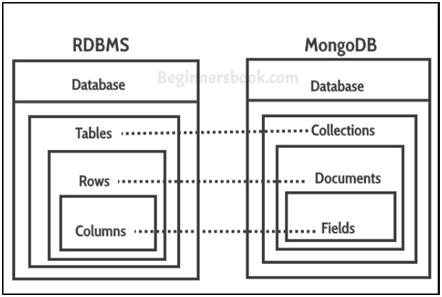
\includegraphics{src/public/oppar/mongodb-structure.jpg} \\
Kuva \getImgCount. Kaavio MongoDB:n struktuurista\labimgcite{lamba18}
\medskip


Dokumentti sisältää datan, jossain standardisoidussa formaatissa kuten XML, YAML, JSON ym.
Dokumentit vastaavat karkeasti objektia, eikä niitten pidä sitoutua mihinkään standardi skeemaan, 
eikä niillä tarvitse olla samoja kenttiä.\labciteend{mongodb24j}
\medskip


MongoDB tallettaa tiedot BSON muodossa, joka on binaari edustus JSON formaatista.
tietokannasta dokumentteja voi hakea niiden uniikkien tunnisteiden tai sisällön arvojen perusteella.\labciteend{mongodb24a}
\medskip



